
\paragraph{UC-4 Visualizzazione degli utenti registrati presso il sistema}
\begin{figure}[H]
    \centering
      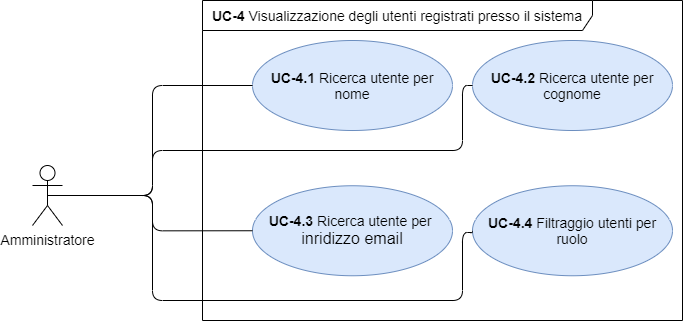
\includegraphics[scale=0.50]{src/CasiDUso/immagini/VisualizzazioneUtenti.png}
    \caption{Diagramma relativo la visualizzazione degli utenti registrati nel sistema}
\end{figure}


\begin{itemize}
	\item \textbf{Attore primario:} amministratore; 

	\item \textbf{Descrizione:} l'amministratore può visualizzare una lista di tutti gli utenti registrati presso il sistema, con funzionalità di ricerca specifica per nome, cognome o indirizzo email oppure filtraggio per il ruolo;

	\item \textbf{Precondizioni:} l'amministratore è autenticato presso l'applicazione web;

	\item \textbf{Postcondizioni:} l'amministratore visualizza l'elenco degli utenti o l'utente desiderato;

	\item \textbf{Scenario principale:}
	      \begin{enumerate}
		      \item l'amministratore accede alla funzionalità di visualizzazione e ricerca utenti;
		      \item l'amministratore visualizza una lista di tutti gli utenti;
		      \item l'amministratore può ricercare un determinato utente per nome/cognome/email (UC-4.1, UC-4.2, UC-4.3);
		      \item l'amministratore può filtrare la lista per i diversi ruoli riconosciuti nel sistema (UC-4,4).
	      \end{enumerate}
\end{itemize}

    \paragraph{UC-4.1 Ricerca utente per nome}
    \begin{itemize}
        \item \textbf{Attore primario:} amministratore; 
    
        \item \textbf{Descrizione:} l'amministratore può visualizzare uno o più utenti corrispondenti ad un nome ricercato;
    
        \item \textbf{Precondizioni:} l'amministratore visualizza la lista di tutti gli utenti del sistema;
    
        \item \textbf{Postcondizioni:} l'amministratore visualizza l'utente o la lista di utenti che possiedono il nome ricercato;
    
        \item \textbf{Scenario principale:}
              \begin{enumerate}
                  \item l'amministratore digita il nome nell'apposita barra di ricerca;
                  \item vengono visualizzati l'utente o la lista di utenti corrispondenti;
                  \item se non viene riconosciuta nessuna voce corrispondente alla stringa digitata non verrà visualizzato alcun utente.
              \end{enumerate}
    \end{itemize}

    \paragraph{UC-4.2 Ricerca utente per cognome}
    \begin{itemize}
        \item \textbf{Attore primario:} amministratore; 
    
        \item \textbf{Descrizione:} l'amministratore può visualizzare uno o più utenti corrispondenti ad un cognome ricercato;
    
        \item \textbf{Precondizioni:} l'amministratore visualizza la lista di tutti gli utenti del sistema;
    
        \item \textbf{Postcondizioni:} l'amministratore visualizza l'utente o la lista di utenti che possiedono il cognome ricercato;
    
        \item \textbf{Scenario principale:}
              \begin{enumerate}
                  \item l'amministratore digita un cognome nell'apposita barra di ricerca;
                  \item vengono visualizzati l'utente o la lista di utenti corrispondenti;
                  \item se non viene riconosciuta nessuna voce corrispondente alla stringa digitata non verrà visualizzato alcun utente.
              \end{enumerate}
    \end{itemize}


    \paragraph{UC-4.3 Ricerca utente per indirizzo email}
    \begin{itemize}
        \item \textbf{Attore primario:} amministratore; 
    
        \item \textbf{Descrizione:} l'amministratore può visualizzare l'utente corrispondente ad un indirizzo email inserito.
    
        \item \textbf{Precondizioni:} l'amministratore visualizza la lista di tutti gli utenti del sistema.
    
        \item \textbf{Postcondizioni:} l'amministratore visualizza l'utente associato all'indirizzo email.
    
        \item \textbf{Scenario principale:}
              \begin{enumerate}
                  \item l'amministratore digita un indirizzo email nell'apposita barra di ricerca;
                  \item viene visualizzato l'utente corrispondente;
                  \item se non viene riconosciuta nessuna voce corrispondente alla stringa digitata non verrà visualizzato alcun utente.
              \end{enumerate}
    \end{itemize}

    \paragraph{UC-4.4 Filtraggio utente per ruolo}
    \begin{itemize}
        \item \textbf{Attore primario:} amministratore; 
    
        \item \textbf{Descrizione:} l'amministratore può filtrare la liste degli utenti visualizzando solo quelli corrispondenti ad un determinato ruolo, che può essere amministratore, dipendente o igienizatore.
    
        \item \textbf{Precondizioni:} l'amministratore visualizza la lista di tutti gli utenti del sistema.
    
        \item \textbf{Postcondizioni:} l'amministratore visualizza la lista di utenti appartenente al ruolo selezionato.
    
        \item \textbf{Scenario principale:}
              \begin{enumerate}
                  \item l'amministratore seleziona un ruolo tra quelli disponibili nell'apposito campo;
                  \item viene visualizzata la lista di utenti corrispondente.
              \end{enumerate}
    \end{itemize}

%diagramma
\paragraph{UC-5 Aggiunta di un nuovo utente nel sistema}
\begin{itemize}
    \item \textbf{Attore primario:} amministratore; 

    \item \textbf{Descrizione:} l'amministratore avvia la procedura per aggiungere un nuovo utente nel sistema inserendo il rispettivo ruolo e l'indirizzo email a cui verrà inviato un link per completare la registrazione (UC-29 Completamento della registrazione da parte del nuovo utente).

    \item \textbf{Precondizioni:} l'amministratore è  autenticato presso l'applicazione web.

    \item \textbf{Postcondizioni:} il sistema ha inviato correttamente il link di registrazione presso l'indirizzo email inserito.

    \item \textbf{Scenario principale:}
          \begin{enumerate}
              \item l'amministratore accede alla funzionalità di aggiunta di un nuovo utente;
              \item l'amministratore seleziona il ruolo da assegnare al nuovo utente (UC-5.1 Selezione ruolo del nuovo utente);
              \item l'amministratore inserisce l'indirizzo email dell'utente da registrare (UC-5.2 Inserimento email del nuovo utente);
              \item l'amministratore conferma l'inserimento;
              \item il sistema elabora la richiesta: se l'indirizzo email è valido verrà inviata una mail contenente il link, altrimenti verrà visualizzato un messaggio di errore (UC-9 Errore: email non valida).
          \end{enumerate}
\end{itemize}

    \paragraph{UC-5.1 Selezione ruolo del nuovo utente}
    \begin{itemize}
        \item \textbf{Attore primario:} amministratore; 
    
        \item \textbf{Descrizione:} l'amministratore può selezionare il ruolo da assegnare al nuovo utente da aggiungere, che può essere dipendente, igienizzatore o amministratore. A seconda del ruolo dipenderà la tipologia di accesso al sistema e le funzionalità permesse.
    
        \item \textbf{Precondizioni:} l'amministratore ha avviato la funzionaliità di aggiunta di un nuovo utente.
    
        \item \textbf{Postcondizioni:} il ruolo da assegnare al nuovo utente è stato selezionato.
    
        \item \textbf{Scenario principale:}
              \begin{enumerate}
                  \item l'amministratore seleziona il ruolo da assegnare tra quelli disponibili.
              \end{enumerate}
    \end{itemize}

    \paragraph{UC-5.2 Inserimento email del nuovo utente}
    \begin{itemize}
        \item \textbf{Attore primario:} amministratore; 
    
        \item \textbf{Descrizione:} l'amministratore inserisce nell'apposito campo l'indirizzo email a cui inviare il link di registrazione.
    
        \item \textbf{Precondizioni:} l'amministratore ha avviato la funzionaliità di aggiunta di un nuovo utente.
    
        \item \textbf{Postcondizioni:} l'indirizzo email è stato correttamente inserito.
    
        \item \textbf{Scenario principale:}
              \begin{enumerate}
                  \item l'amministratore digita l'indirizzo email nell'apposito campo di inserimento.
              \end{enumerate}
        \item \textbf{Estensioni:}
              \begin{itemize}
                    \item UC-9 Errore: email non valida.
            \end{itemize}
    \end{itemize}

%diagramma
\paragraph{UC-6 Visualizzazione dati utente}
\begin{itemize}
	\item \textbf{Attore primario:} amministratore.

	\item \textbf{Descrizione:} l'amministratore può visualizzare i dati degli utenti registrati nel sistema, quali nome (UC-6.1), cognome (UC-6.2), ruolo (UC-6.3), email (UC-6.4), password (UC-6.5), storico degli accessi (UC-6.6) e storico dell'utilizzo delle postazioni (UC-6.7).
	
	\item \textbf{Precondizioni:} l'amministratore è autenticato presso il sistema.

	\item \textbf{Postcondizioni:} l'amministratore visualizza i dati relativi al profilo dell'utente selezionato.

	\item \textbf{Scenario principale:}
	\begin{enumerate}
    	\item  l'amministratore seleziona l'utente di cui vuole visualizzare i dati;
    	\item  l'amministrtore visualizza i dati dell'utente.
	\end{enumerate}
\end{itemize}

    \paragraph{UC-6.1 Visualizzazione nome utente}
    \begin{itemize}
        \item \textbf{Attore primario:} amministratore.
        
        \item \textbf{Descrizione:} l'amministratore può visualizzare il nome dell'utente registrato, all'interno del relativo profilo.
        
        \item \textbf{Precondizioni:} l'amministratore ha selezionato l'utente di cui vuole visualizzare il profilo.
    
        \item \textbf{Postcondizioni:} il nome dell'utente è visibile all'interno del relativo profilo.
    
        \item \textbf{Scenario principale:}
        \begin{enumerate}
            \item  l'amministratore seleziona l'utente di cui vuole visualizzare i dati;
            \item  l'amministratore visualizza il nome dell'utente.
        \end{enumerate}
    \end{itemize}

    \paragraph{UC-6.2 Visualizzazione cognome utente}
    \begin{itemize}
        \item \textbf{Attore primario:} amministratore.
        
        \item \textbf{Descrizione:} l'amministratore può visualizzare il cognome dell'utente registrato, all'interno del relativo profilo.
        
        \item \textbf{Precondizioni:} l'amministratore ha selezionato l'utente di cui vuole visualizzare il profilo.
    
        \item \textbf{Postcondizioni:} il cognome dell'utente è visibile all'interno del relativo profilo.
    
        \item \textbf{Scenario principale:}
        \begin{enumerate}
            \item  l'amministratore seleziona l'utente di cui vuole visualizzare i dati;
            \item  l'amministratore visualizza il cognome dell'utente.
        \end{enumerate}
    \end{itemize}

    \paragraph{UC-6.3 Visualizzazione ruolo utente}
    \begin{itemize}
        \item \textbf{Attore primario:} amministratore.
        
        \item \textbf{Descrizione:} l'amministratore può visualizzare il ruolo dell'utente registrato, all'interno del relativo profilo.
        
        \item \textbf{Precondizioni:} l'amministratore ha selezionato l'utente di cui vuole visualizzare il profilo.
    
        \item \textbf{Postcondizioni:} il ruolo dell'utente è visibile all'interno del relativo profilo.
    
        \item \textbf{Scenario principale:}
        \begin{enumerate}
            \item  l'amministratore seleziona l'utente di cui vuole visualizzare i dati;
            \item  l'amministratore visualizza il ruolo dell'utente.
        \end{enumerate}
    \end{itemize}

    \paragraph{UC-6.4 Visualizzazione email utente}
    \begin{itemize}
        \item \textbf{Attore primario:} amministratore.
        
        \item \textbf{Descrizione:} l'amministratore può visualizzare l'indirizzo email dell'utente registrato, all'interno del relativo profilo.
        
        \item \textbf{Precondizioni:} l'amministratore ha selezionato l'utente di cui vuole visualizzare il profilo.
    
        \item \textbf{Postcondizioni:} l'indirizzo email dell'utente è visibile all'interno del relativo profilo.
    
        \item \textbf{Scenario principale:}
        \begin{enumerate}
            \item  l'amministratore seleziona l'utente di cui vuole visualizzare i dati;
            \item  l'amministratore visualizza l'indirizzo email dell'utente.
        \end{enumerate}
    \end{itemize}

    \paragraph{UC-6.5 Visualizzazione password utente}
    \begin{itemize}
        \item \textbf{Attore primario:} amministratore.
        
        \item \textbf{Descrizione:} l'amministratore può visualizzare la password dell'utente registrato, all'interno del relativo profilo.
        
        \item \textbf{Precondizioni:} l'amministratore ha selezionato l'utente di cui vuole visualizzare il profilo.
    
        \item \textbf{Postcondizioni:} la password dell'utente è visibile all'interno del relativo profilo.
    
        \item \textbf{Scenario principale:}
        \begin{enumerate}
            \item  l'amministratore seleziona l'utente di cui vuole visualizzare i dati;
            \item  l'amministratore visualizza la password dell'utente.
        \end{enumerate}
    \end{itemize}
    

    \paragraph{UC-6.6 Visualizzazione storico accessi utente}
    \begin{itemize}
        \item \textbf{Attore primario:} amministratore.
        
        \item \textbf{Descrizione:} l'amministratore può visualizzare uno storico con data e ora di tutti gli accessi effettuati dall'utente presso il sistema tramite applicazione mobile.
        
        \item \textbf{Precondizioni:} l'amministratore ha selezionato l'utente di cui vuole visualizzare il profilo.
    
        \item \textbf{Postcondizioni:} l'amministratore visualizza lo storico degli accessi da parte dell'utente.
    
        \item \textbf{Scenario principale:}
        \begin{enumerate}
            \item  l'amministratore seleziona l'utente di cui vuole visualizzare i dati;
            \item  l'amministratore seleziona la funzionalità di visualizzazione dello storico degli accessi;
            \item l'amministratore visualizza un elenco con data e ora di tutti gli accessi effettuati dall'utente.
        \end{enumerate}
    \end{itemize}

    \paragraph{UC-6.7 Visualizzazione storico dell'utilizzo postazioni}
    \begin{itemize}
        \item \textbf{Attore primario:} amministratore.
        
        \item \textbf{Descrizione:} l'amministratore può visualizzare uno storico con data, ora e codice postazione, di tutti gli utilizzi delle postazioni effettuati dall'utente e registrati presso il sistema tramite applicazione mobile.
        
        \item \textbf{Precondizioni:} l'amministratore ha selezionato l'utente di cui vuole visualizzare il profilo.
    
        \item \textbf{Postcondizioni:} l'amministratore visualizza lo storico dell'utilizzo delle postazioni da parte dell'utente.
    
        \item \textbf{Scenario principale:}
        \begin{enumerate}
            \item  l'amministratore seleziona l'utente di cui vuole visualizzare i dati;
            \item  l'amministratore seleziona la funzionalità di visualizzazione dello storico relativo all'utilizzo postazioni;
            \item l'amministratore visualizza un elenco con data, ora e codice postazione di ogni utilizzo effettuato dall'utente.
        \end{enumerate}
    \end{itemize}

%diagramma
\paragraph{UC-7 Modifica dati utente}
\begin{itemize}
	\item \textbf{Attore primario:} amministratore.

	\item \textbf{Descrizione:} l'amministratore può modificare il ruolo (UC-7.1) e l'indirizzo email (UC-7.2) dell'utente selezionato.
	
	\item \textbf{Precondizioni:} l'amministratore è autenticato presso il sistema.

	\item \textbf{Postcondizioni:} l'amministratore ha modificato uno dei campi dati permessi dell'utente.

	\item \textbf{Scenario principale:}
	\begin{enumerate}
    	\item  l'amministratore seleziona l'utente di cui vuole modificare i dati;
    	\item  l'amministratore seleziona il dato da modificare;
    	\item l'amministratore modifica il dato dell'utente.
    	\item l'amministratore conferma la modifica effettuata.
	\end{enumerate}
\end{itemize}
    
    \paragraph{UC-7.1 Modifica ruolo utente}
    \begin{itemize}
        \item \textbf{Attore primario:} amministratore.
    
        \item \textbf{Descrizione:} l'amministratore può modificare il ruolo dell'utente selezionato.
        
        \item \textbf{Precondizioni:} l'amministratore ha selezionato l'utente di cui vuole modificare il ruolo.
    
        \item \textbf{Postcondizioni:} l'amministratore ha modificato il ruolo dell'utente.
    
        \item \textbf{Scenario principale:}
        \begin{enumerate}
            \item  l'amministratore seleziona il nuovo ruolo da assegnare all'utente tra quelli disponibili.
            \item l'amministratore conferma la selezione;
            \item il sistema elabora la richiesta e completa la modifica.
        \end{enumerate}
    \end{itemize}
    
    \paragraph{UC-7.2 Modifica email utente}
    \begin{itemize}
        \item \textbf{Attore primario:} amministratore.
    
        \item \textbf{Descrizione:} l'amministratore può modificare l'indirizzo email dell'utente selezionato.
        
        \item \textbf{Precondizioni:} l'amministratore ha selezionato l'utente di cui vuole modificare l'indirizzo email.
    
        \item \textbf{Postcondizioni:} l'amministratore ha modificato l'indirizzo email dell'utente.
    
        \item \textbf{Scenario principale:}
        \begin{enumerate}
            \item  l'amministratore seleziona la funzionalità di modifica del campo relativo all'indirizzo email dell'utente;
            \item l'amministratore digita il nuovo indirizzo email nell'apposito campo;
            \item l'amministratore conferma la modifica;
            \item il sistema elabora la richiesta ed attua la modifica. In caso contrario restituisce un messaggio di errore (UC-9 Errore: email non valida) e non completa la modifica.
        \end{enumerate}
        \item \textbf{Estensioni:}
              \begin{itemize}
                    \item UC-9 Errore: email non valida.
            \end{itemize}
    \end{itemize}


\paragraph{UC-9 Errore: email non valida}
\begin{itemize}
	\item \textbf{Attore primario:} amministratore;

	\item \textbf{Descrizione:} l'amministratore ha provato a registrare un nuovo utente ma la registrazione non è andata a buon fine poiché l'indirizzo e-mail risultava già censito (UC-9.1 Errore: email già presente nel sistema) o inadeguato ai criteri stabiliti per la creazione di un indirizzo e-mail (UC-9.2 Errore: caratteri email non validi);

	\item \textbf{Precondizioni:} l'amministratore ha inserito un indirizzo e-mail non valido durante la registrazione ed ha inviato i dati al sistema;

	\item \textbf{Postcondizioni:} il sistema restituisce un messaggio d'errore esplicativo e non completa la registrazione del nuovo utente;

	\item \textbf{Scenario principale:}
	      \begin{enumerate}
		      \item il sistema elabora la richiesta ricevuta;
		      \item il sistema restituisce un messaggio d'errore esplicativo e non completa la registrazione del nuovo utente.
	      \end{enumerate}
\end{itemize}

    \paragraph{UC-9.1 Errore: email già presente nel sistema}
    \begin{itemize}
        \item \textbf{Attore primario:} amministratore;
    
        \item \textbf{Descrizione:} l'amministratore ha provato a registrare un nuovo utente ma la registrazione non è andata a buon fine poiché l'indirizzo e-mail inserito è già associato ad un altro utente all'interno del sistema;
    
        \item \textbf{Precondizioni:} l'amministratore ha inserito un indirizzo e-mail già utilizzato da un altro utente durante la registrazione e ha inviato i dati al sistema;
    
        \item \textbf{Postcondizioni:} il sistema restituisce un messaggio d'errore esplicativo e non completa la registrazione del nuovo utente;
    
        \item \textbf{Scenario principale:}
              \begin{enumerate}
                  \item il sistema elabora la richiesta ricevuta;
                  \item il sistema restituisce un messaggio d'errore esplicativo e non completa la registrazione del nuovo utente.
              \end{enumerate}
    \end{itemize}

    \paragraph{UC-9.2 Errore: caratteri email non validi}
    \begin{itemize}
        \item \textbf{Attore primario:} amministratore;
    
        \item \textbf{Descrizione:} l'amministratore ha provato a registrare un nuovo utente ma la registrazione non è andata a buon fine poiché l'indirizzo e-mail inserito contiene dei caratteri speciali che non rispettano i criteri di inserimento di un nuovo indirizzo e-mail;
    
        \item \textbf{Precondizioni:} l'amministratore ha inserito un indirizzo e-mail che contiene dei caratteri non validi durante la registrazione ed ha inviato i dati al sistema;
    
        \item \textbf{Postcondizioni:} il sistema restituisce un messaggio d'errore esplicativo e non completa la registrazione del nuovo utente;
    
        \item \textbf{Scenario principale:}
              \begin{enumerate}
                  \item il sistema elabora la richiesta ricevuta;
                  \item il sistema restituisce un messaggio d'errore esplicativo e non completa la registrazione del nuovo utente.
              \end{enumerate}
    \end{itemize}

\paragraph{UC-10 Rimozione di un utente dal sistema}
\begin{itemize}
    \item \textbf{Attore primario:} amministratore;

    \item \textbf{Descrizione:} l'amministratore può rimuovere un utente selezionato dal sistema;

    \item \textbf{Precondizioni:} l'amministratore è autenticato presso l'applicazione web;

    \item \textbf{Postcondizioni:} l'utente non è più registrato presso il sistema;

    \item \textbf{Scenario principale:}
          \begin{enumerate}
              \item l'amministratore seleziona l'utente che intende rimuovere;
              \item l'amministratore seleziona la funzionalità di rimozione dell'utente;
              \item il sistema elabora correttamente la richiesta e rimuove l'utente.
          \end{enumerate}
\end{itemize}